\documentclass[11pt,a4paper]{article}
\usepackage{fontspec}
\setmainfont{Cambria}
\usepackage[spanish,es-nodecimaldot,es-noshorthands]{babel}
\usepackage[margin=2.3cm]{geometry}
\usepackage{amsmath,amssymb}
\usepackage{booktabs,array,longtable}
\usepackage{graphicx}
\graphicspath{{../Figuras/}}
\usepackage{xcolor}
\usepackage{float}
\usepackage{fancyhdr}
\usepackage[hidelinks]{hyperref}
% Fuentes matemáticas a partir de los tamaños base de 10 pt (escaladas)
\DeclareFontShape{OML}{cmm}{m}{it}{<->cmmi10}{}
\DeclareFontShape{OML}{cmm}{b}{it}{<->cmmi10}{}
\DeclareFontShape{OMS}{cmsy}{m}{n}{<->cmsy10}{}
\DeclareFontShape{OMS}{cmsy}{b}{n}{<->cmsy10}{}
\DeclareFontShape{OT1}{cmr}{m}{n}{<->cmr10}{}
\DeclareFontShape{OT1}{cmr}{bx}{n}{<->cmr10}{}
\definecolor{verde}{RGB}{0,128,60}
\definecolor{rojo}{RGB}{200,30,30}
\setlength{\parindent}{0pt}
\setlength{\parskip}{6pt}
\pagestyle{fancy}\fancyhf{}
\lhead{\small Memoria de cálculo -- Viga presforzada}
\rhead{\small L = 35.0 m}
\cfoot{\thepage}
\title{\textbf{Diseño de viga de hormigón presforzado}\\[4pt]\large Memoria de cálculo -- Puente de luz L = 35.0 m}
\date{18 de noviembre de 2026}
\author{}
\begin{document}
\maketitle
\thispagestyle{fancy}
\tableofcontents
\newpage
\textbf{Unidades:} kg, cm (sección), m (luz y abscisas $x$), kg/m (cargas), kg$\cdot$m (momentos), kg/cm$^2$ (esfuerzos).\\
\textbf{Convención de signos:} compresión negativa ($-$), tracción positiva ($+$). Fibra 1 = superior, fibra 2 = inferior.
Excentricidades positivas hacia abajo del centro de gravedad. Las abscisas $x$ se miden desde el apoyo izquierdo.


\section{Datos de diseño}
\begin{center}
\begin{tabular}{llr}
\toprule
Parámetro & Símbolo & Valor \\
\midrule
Luz de cálculo (simplemente apoyada) & $L$ & 35.00 m \\
Resistencia del hormigón & $f'_c$ & 420.00 kg/cm$^2$ \\
Resistencia en la transferencia ($f'_{ci} = 0.70\,f'_c$) & $f'_{ci}$ & 294.00 kg/cm$^2$ \\
Peso específico del hormigón & $\gamma_c$ & 2\,400 kg/m$^3$ \\
Pérdidas de presfuerzo & -- & 18.0 \% \\
Fibra inferior al cable resultante (en $L/2$) & $d_2$ & 17.00 cm \\
\midrule
Losa & $q_{losa}$ & 1\,260.00 kg/m \\
Acera & $q_{acera}$ & 128.00 kg/m \\
Postes y pasamanos & $q_{parantes}$ & 17.55 kg/m \\
Carpeta asfáltica & $q_{asfalto}$ & 241.50 kg/m \\
Carga viva & $q_L$ & 1\,200.00 kg/m \\
\midrule
Peso propio asumido (predimensionamiento) & $q_{G,asum}$ & 1\,000.00 kg/m \\
Coeficiente $h = L/k$ & $k_L$ & 16 \\
Coeficiente $h = k\sqrt{M}$ & $k_M$ & 0.4 \\
\bottomrule
\end{tabular}
\end{center}


\section{Predimensionamiento de la sección}
Para el predimensionamiento se asume el peso propio $q_{G,asum} = 1\,000.00$ kg/m:
\begin{align*}
q_T &= q_D + q_{G,asum} + q_L = 1\,647.05 + 1\,000.00 + 1\,200.00 = 3\,847.05\ \text{kg/m}\\
M_G &= \frac{q_{G,asum} L^2}{8} = \frac{(1\,000.00)(35.0)^2}{8} = 153\,125.00\ \text{kg}\cdot\text{m}\\
M_T &= \frac{q_T L^2}{8} = \frac{(3\,847.05)(35.0)^2}{8} = 589\,079.53\ \text{kg}\cdot\text{m}
\end{align*}

\subsection{Altura}
\begin{center}
\renewcommand{\arraystretch}{1.9}
\begin{tabular}{lr}
\toprule
Criterio & $h$ \\
\midrule
$h = \dfrac{L}{k} = \dfrac{3\,500\ \text{cm}}{16}$ & 218.75 cm \\
$h = \dfrac{L}{25} + 10 = \dfrac{3\,500}{25} + 10$ & 150.00 cm \\
$h = k\sqrt{M_T} = 0.4\sqrt{589\,079.53}$ & 307.01 cm \\
$h = 0.07\,L = 0.07\,(3\,500)$ & 245.00 cm \\
\midrule
\textbf{Promedio (altura recomendada)} & \textbf{230.19 cm} \\
\bottomrule
\end{tabular}
\end{center}


\subsection{Área de hormigón requerida}
Con $f_c = 0.45\,f'_c = 0.45\,(420.00) = 189.00$ kg/cm$^2$, $h = 230.19$ cm, $M_L = M_T - M_G = 435\,954.53$ kg$\cdot$m
y $M_G/M_T = 0.260$:
\begin{align*}
A_{c,1} &= \frac{4\,M_L}{f_c\,h} = \frac{4\,(435\,954.53\times10^2)}{(189.00)(230.19)} = 4\,008.25\ \text{cm}^2 \\
A_{c,2} &= \frac{3\,M_T}{f_c\,h} = \frac{3\,(589\,079.53\times10^2)}{(189.00)(230.19)} = 4\,062.08\ \text{cm}^2
\end{align*}
Como $0.20 \le M_G/M_T \le 0.30$ (entre ambos casos), se adopta el mayor de las dos expresiones. \quad $\Rightarrow\ A_{c,req} = \textbf{4\,062.08}$ cm$^2$.

\subsection{Recomendaciones para el dibujo de la sección}
\begin{itemize}
\item Altura: $h \approx 230.19$ cm.
\item Área de hormigón: $A_c \ge 4\,062.08$ cm$^2$.
\item Ancho de alma: $b_w = 16$ a $20$ cm (el menor posible). Donde existan mayores compresiones debe disponerse mayor sección de hormigón.
\end{itemize}


\section{Iteraciones de la sección transversal}
Se partió de la sección T obtenida del predimensionamiento y se modificó la sección hasta cumplir los esfuerzos
admisibles de $f_1$ y $f_2$ en las etapas inicial y final. En cada iteración se recalcularon con el peso propio real
($q_G = A\,\gamma_c$) los momentos, el presfuerzo $F_0$, $F$, la excentricidad $e$, los esfuerzos y la eficiencia $Q$.
Se registraron 2 iteraciones. 

\begin{center}\small
\begin{tabular}{clrrcl}
\toprule
N.\textsuperscript{o} & Sección [cm] & $A$ [cm$^2$] & $q_G$ [kg/m] & $Q$ & Estado \\
\midrule
1 & T  (B=40, t=16, bw=16, h=230) & 4\,064 & 975.4 & 0.379 & \textcolor{rojo}{\textbf{No cumple}} \\
2 & I  (bs=45, ts=16, bw=16, bi=80, ti=21, h=230) & 5\,488 & 1\,317.1 & 0.489 & \textcolor{verde}{Adoptada} \\
\bottomrule
\end{tabular}
\end{center}

\begin{center}\small\setlength{\tabcolsep}{4.5pt}
\begin{tabular}{ccrrrrrrr}
\toprule
& & & & & \multicolumn{2}{c}{Inicial [kg/cm$^2$]} & \multicolumn{2}{c}{Final [kg/cm$^2$]} \\
\cmidrule(lr){6-7}\cmidrule(lr){8-9}
N.\textsuperscript{o} & Exc. & $F_0$ [kg] & $F$ [kg] & $e$ [cm] & $f_1$ & $f_2$ & $f_1$ & $f_2$ \\
\midrule
1 & NR & 647\,858 & 531\,031 & 70.47 & 0.00 & \textcolor{rojo}{\textbf{-349.56}} & \textcolor{rojo}{\textbf{-240.22}} & 0.00 \\
2 & R & 533\,540 & 437\,328 & 81.45 & -9.10 & -163.17 & -186.16 & 0.00 \\
\bottomrule
\end{tabular}
\end{center}
Exc.: NR = excentricidad no restringida, R = restringida. Admisibles: inicial $-176.40 \le f \le 0$, final
$-189.00 \le f \le 0$ kg/cm$^2$. Los valores en \textcolor{rojo}{\textbf{rojo}} no cumplen.


\subsection{Iteración 1: T  (B=40, t=16, bw=16, h=230)}
\begin{minipage}[c]{0.42\textwidth}
\centering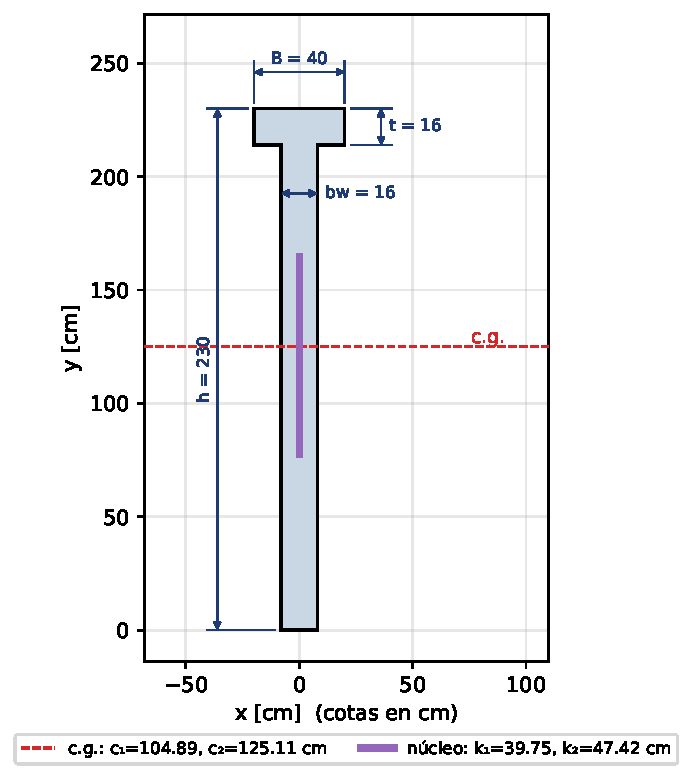
\includegraphics[width=\linewidth]{iteracion_1.pdf}
\end{minipage}\hfill
\begin{minipage}[c]{0.54\textwidth}\small
\begin{tabular}{lr}
\toprule
$A$ & 4\,064.00 cm$^2$ \\
$c_1$ / $c_2$ & 104.89 / 125.11 cm \\
$I$ & 20\,211\,865 cm$^4$ \\
$k_1$ / $k_2$ & 39.75 / 47.42 cm \\
$q_G = A\,\gamma_c$ & 975.36 kg/m \\
$M_G$ / $M_T$ & 149\,352.00 / 585\,306.53 kg$\cdot$m \\
$e_{max} = c_2 - d_2$ & 108.11 cm \\
$Q = (k_1 + k_2)/h$ & 0.379 \\
\bottomrule
\end{tabular}
\end{minipage}

Como $e = 70.47$ cm $\le e_{max} = 108.11$ cm, la excentricidad es \textbf{no restringida}:
$F = 531\,031.49$ kg, $F_0 = 647\,858.41$ kg.

\textbf{Etapa inicial (F\textsubscript{0} + M\textsubscript{G}):}
\begin{align*}
f_1 &= -\frac{F_0}{A} + \frac{F_0\,e}{S_1} - \frac{M_G}{S_1}
= -\frac{647\,858.41}{4\,064.00} + \frac{(647\,858.41)(70.47)}{192\,696.26} - \frac{14\,935\,200}{192\,696.26} = \textbf{0.00}\ \text{kg/cm}^2\\
f_2 &= -\frac{F_0}{A} - \frac{F_0\,e}{S_2} + \frac{M_G}{S_2}
= -\frac{647\,858.41}{4\,064.00} - \frac{(647\,858.41)(70.47)}{161\,552.45} + \frac{14\,935\,200}{161\,552.45} = \textbf{-349.56}\ \text{kg/cm}^2
\end{align*}
\textbf{Etapa final (F + M\textsubscript{T}):}
\begin{align*}
f_1 &= -\frac{F}{A} + \frac{F\,e}{S_1} - \frac{M_T}{S_1}
= -\frac{531\,031.49}{4\,064.00} + \frac{(531\,031.49)(70.47)}{192\,696.26} - \frac{58\,530\,653}{192\,696.26} = \textbf{-240.22}\ \text{kg/cm}^2\\
f_2 &= -\frac{F}{A} - \frac{F\,e}{S_2} + \frac{M_T}{S_2}
= -\frac{531\,031.49}{4\,064.00} - \frac{(531\,031.49)(70.47)}{161\,552.45} + \frac{58\,530\,653}{161\,552.45} = \textbf{0.00}\ \text{kg/cm}^2
\end{align*}

\textcolor{rojo}{\textbf{No cumple}}:\begin{itemize}\item f$_2$ inicial = -349.56 kg/cm$^2$ $<$ -176.40 kg/cm$^2$ (excede la compresión admisible)\item f$_1$ final = -240.22 kg/cm$^2$ $<$ -189.00 kg/cm$^2$ (excede la compresión admisible)\end{itemize}Se descarta y se modifica la sección. Eficiencia: SECCIÓN PESADA (Q $<$ 0.45).


\subsection{Iteración 2: I  (bs=45, ts=16, bw=16, bi=80, ti=21, h=230)}
\begin{minipage}[c]{0.42\textwidth}
\centering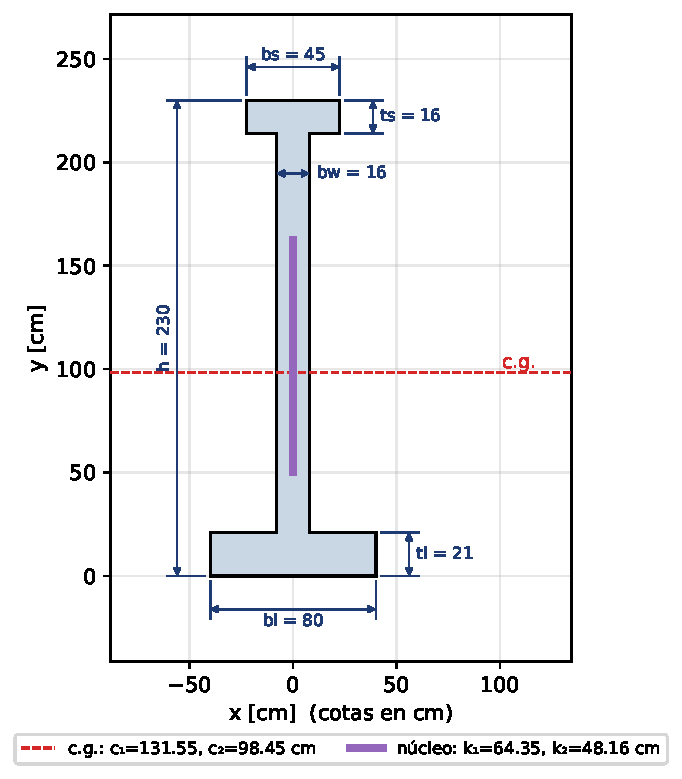
\includegraphics[width=\linewidth]{iteracion_2.pdf}
\end{minipage}\hfill
\begin{minipage}[c]{0.54\textwidth}\small
\begin{tabular}{lr}
\toprule
$A$ & 5\,488.00 cm$^2$ \\
$c_1$ / $c_2$ & 131.55 / 98.45 cm \\
$I$ & 34\,768\,806 cm$^4$ \\
$k_1$ / $k_2$ & 64.35 / 48.16 cm \\
$q_G = A\,\gamma_c$ & 1\,317.12 kg/m \\
$M_G$ / $M_T$ & 201\,684.00 / 637\,638.53 kg$\cdot$m \\
$e_{max} = c_2 - d_2$ & 81.45 cm \\
$Q = (k_1 + k_2)/h$ & 0.489 \\
\bottomrule
\end{tabular}
\end{minipage}

Como $e = 87.54$ cm $> e_{max} = 81.45$ cm, la excentricidad es \textbf{restringida}:
$F = \dfrac{M_T}{e_{max} + k_1} = 437\,327.75$ kg, $F_0 = \alpha F = 533\,539.85$ kg, $e = e_{max} = 81.45$ cm.

\textbf{Etapa inicial (F\textsubscript{0} + M\textsubscript{G}):}
\begin{align*}
f_1 &= -\frac{F_0}{A} + \frac{F_0\,e}{S_1} - \frac{M_G}{S_1}
= -\frac{533\,539.85}{5\,488.00} + \frac{(533\,539.85)(81.45)}{264\,310.74} - \frac{20\,168\,400}{264\,310.74} = \textbf{-9.10}\ \text{kg/cm}^2\\
f_2 &= -\frac{F_0}{A} - \frac{F_0\,e}{S_2} + \frac{M_G}{S_2}
= -\frac{533\,539.85}{5\,488.00} - \frac{(533\,539.85)(81.45)}{353\,144.82} + \frac{20\,168\,400}{353\,144.82} = \textbf{-163.17}\ \text{kg/cm}^2
\end{align*}
\textbf{Etapa final (F + M\textsubscript{T}):}
\begin{align*}
f_1 &= -\frac{F}{A} + \frac{F\,e}{S_1} - \frac{M_T}{S_1}
= -\frac{437\,327.75}{5\,488.00} + \frac{(437\,327.75)(81.45)}{264\,310.74} - \frac{63\,763\,853}{264\,310.74} = \textbf{-186.16}\ \text{kg/cm}^2\\
f_2 &= -\frac{F}{A} - \frac{F\,e}{S_2} + \frac{M_T}{S_2}
= -\frac{437\,327.75}{5\,488.00} - \frac{(437\,327.75)(81.45)}{353\,144.82} + \frac{63\,763\,853}{353\,144.82} = \textbf{0.00}\ \text{kg/cm}^2
\end{align*}

\textcolor{verde}{\textbf{Cumple}} con los esfuerzos admisibles $\Rightarrow$ \textbf{sección adoptada}. Eficiencia: DISEÑO EFICIENTE (0.45 $\le$ Q $\le$ 0.55, óptimo Q = 0.50).


\section{Sección transversal adoptada}
Sección: \textbf{I  (bs=45, ts=16, bw=16, bi=80, ti=21, h=230)}, de altura total $h = 230.0$ cm. Corresponde a la \textbf{iteración 2} del registro.

\begin{figure}[H]
\centering
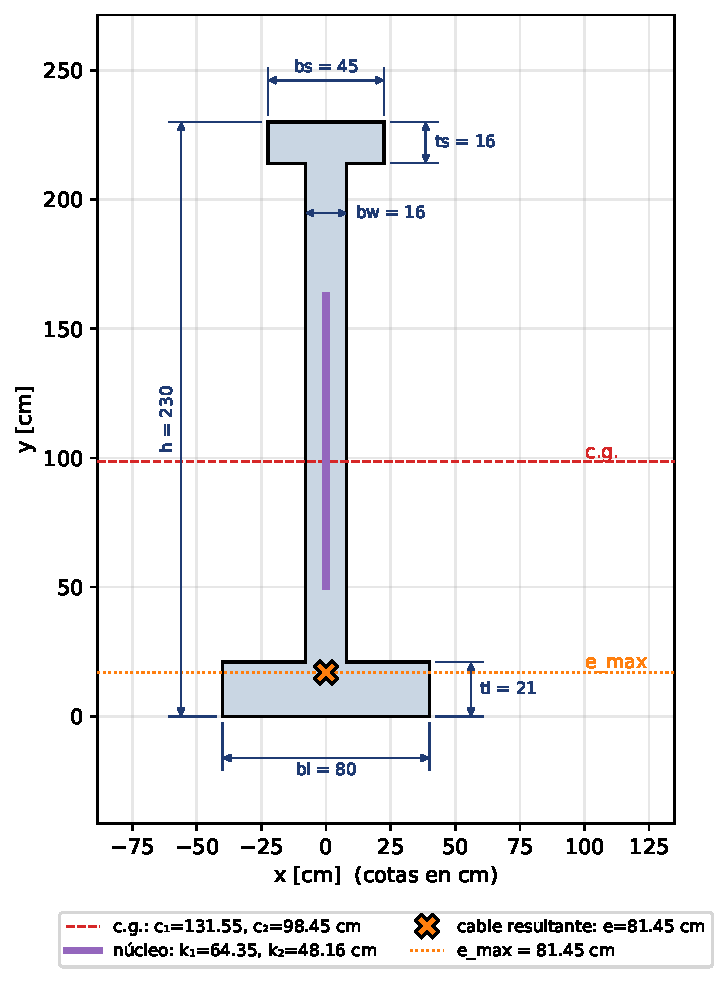
\includegraphics[width=0.6\textwidth]{seccion.pdf}
\caption{Sección transversal: c.g., núcleo central ($k_1$, $k_2$), $e_{max}$ y cable resultante en $L/2$.}
\end{figure}

\begin{center}
\begin{tabular}{llll}
\toprule
Ítem & Recomendado & Adoptado & Observación \\
\midrule
Altura h & 230.2 cm & 230.0 cm & \textcolor{verde}{-0.1 \% respecto al promedio} \\
Área de hormigón $A_c$ & $\ge$ 4,062 cm$^2$ & 5,488 cm$^2$ & \textcolor{verde}{suficiente} \\
Ancho de alma $b_w$ & 16 a 20 cm & 16 cm & \textcolor{verde}{dentro del rango} \\
\bottomrule
\end{tabular}
\end{center}


\section{Propiedades mecánicas}

Las propiedades se obtienen por partes, con $y$ medido desde la fibra inferior:
\begin{center}\footnotesize\setlength{\tabcolsep}{4pt}
\begin{tabular}{lrrrrrrrr}
\toprule
Parte & $b$ [cm] & $h$ [cm] & $A_i$ [cm$^2$] & $y_i$ [cm] & $A_i y_i$ [cm$^3$] & $I_{0,i}$ [cm$^4$] & $d_i$ [cm] & $A_i d_i^2$ [cm$^4$] \\
\midrule
Ala superior & 45.0 & 16.0 & 720.00 & 222.00 & 159\,840.00 & 15\,360.00 & 123.55 & 10\,989\,657.97 \\
Alma & 16.0 & 193.0 & 3\,088.00 & 117.50 & 362\,840.00 & 9\,585\,409.33 & 19.05 & 1\,120\,077.02 \\
Ala inferior & 80.0 & 21.0 & 1\,680.00 & 10.50 & 17\,640.00 & 61\,740.00 & -87.95 & 12\,996\,561.80 \\
\midrule
$\Sigma$ & & & 5\,488.00 & & 540\,320.00 & 9\,662\,509.33 & & 25\,106\,296.79 \\
\bottomrule
\end{tabular}
\end{center}
\begin{align*}
\bar y &= \frac{\Sigma A_i y_i}{\Sigma A_i} = \frac{540\,320.00}{5\,488.00} = 98.45\ \text{cm} \\
I &= \Sigma I_{0,i} + \Sigma A_i d_i^2 = 9\,662\,509.33 + 25\,106\,296.79 = 34\,768\,806.13\ \text{cm}^4
\end{align*}

\begin{align*}
c_1 &= h - \bar y = 131.55\ \text{cm} & c_2 &= \bar y = 98.45\ \text{cm}\\
S_1 &= \frac{I}{c_1} = 264\,310.74\ \text{cm}^3 & S_2 &= \frac{I}{c_2} = 353\,144.82\ \text{cm}^3\\
k_1 &= \frac{I}{A\,c_2} = 64.35\ \text{cm} & k_2 &= \frac{I}{A\,c_1} = 48.16\ \text{cm}\\
r^2 &= \frac{I}{A} = 6\,335.42\ \text{cm}^2 & A &= 5\,488.00\ \text{cm}^2
\end{align*}


\section{Cargas y momentos en el centro de la luz}
El momento en una sección cualquiera es $M(x) = q\,x\,(L-x)/2$; en $x = L/2$ resulta $M = q L^2/8$.
\begin{align*}
q_G &= A\,\gamma_c = (5\,488.00\times10^{-4}\ \text{m}^2)(2\,400\ \text{kg/m}^3) = 1\,317.12\ \text{kg/m}\\
q_D &= q_{losa} + q_{acera} + q_{parantes} + q_{asfalto} = 1\,260.00 + 128.00 + 17.55 + 241.50 = 1\,647.05\ \text{kg/m}\\
q_T &= q_D + q_G + q_L = 1\,647.05 + 1\,317.12 + 1\,200.00 = 4\,164.17\ \text{kg/m}\\
M_G &= \frac{q_G L^2}{8} = \frac{(1\,317.12)(35.0)^2}{8} = 201\,684.00\ \text{kg}\cdot\text{m}\\
M_T &= \frac{q_T L^2}{8} = \frac{(4\,164.17)(35.0)^2}{8} = 637\,638.53\ \text{kg}\cdot\text{m}
\qquad \frac{M_G}{M_T} = 0.32
\end{align*}


\section{Diseño definitivo: fuerzas de presfuerzo y excentricidad}
Condiciones de diseño en el centro de la luz: $f_1 = 0$ en la etapa inicial ($F_0 + M_G$) y $f_2 = 0$ en la etapa final ($F + M_T$).
\begin{align*}
\alpha &= \frac{100}{100 - \%\text{pérdidas}} = \frac{100}{100 - 18.0} = 1.220 &
e_{max} &= c_2 - d_2 = 98.45 - 17.00 = 81.45\ \text{cm}
\end{align*}
\subsection{Excentricidad no restringida}
\begin{align*}
F &= \frac{\alpha M_T - M_G}{\alpha\,(k_1 + k_2)} = \frac{1.220\,(63\,763\,853) - 20\,168\,400}{1.220\,(64.35 + 48.16)} = 419\,805.58\ \text{kg}\\
F_0 &= \alpha F = 1.220\,(419\,805.58) = 512\,162.81\ \text{kg}\\
e &= \frac{M_G}{F_0} + k_2 = \frac{20\,168\,400}{512\,162.81} + 48.16 = 87.54\ \text{cm}
\end{align*}
\subsection{Verificación de la excentricidad}

Como $e = 87.54$ cm $> e_{max} = 81.45$ cm, la altura no permite ubicar la excentricidad calculada
(\textbf{caso dos: excentricidad restringida}). Se fija $e = e_{max}$ y se impone $f_2 = 0$ en la etapa final:
\begin{align*}
F &= \frac{M_T}{e_{max} + k_1} = \frac{63\,763\,853}{81.45 + 64.35} = \textbf{437\,327.75\ kg}\\
F_0 &= \alpha F = 1.220\,(437\,327.75) = \textbf{533\,539.85\ kg}\\
e &= e_{max} = \textbf{81.45\ cm}
\end{align*}

\begin{center}
\begin{tabular}{lr}
\toprule
Fuerza de presfuerzo inicial $F_0$ & \textbf{533\,539.85 kg} \\
Fuerza de presfuerzo final $F$ & \textbf{437\,327.75 kg} \\
Excentricidad del cable resultante en $L/2$, $e$ & \textbf{81.45 cm} \\
Caso & Restringida \\
\bottomrule
\end{tabular}
\end{center}

\section{Análisis de la sección en el centro de la luz}
\textbf{Etapa inicial (F\textsubscript{0} + M\textsubscript{G}):}
\begin{align*}
f_1 &= -\frac{F_0}{A} + \frac{F_0\,e}{S_1} - \frac{M_G}{S_1}
= -\frac{533\,539.85}{5\,488.00} + \frac{(533\,539.85)(81.45)}{264\,310.74} - \frac{20\,168\,400}{264\,310.74} = \textbf{-9.10}\ \text{kg/cm}^2\\
f_2 &= -\frac{F_0}{A} - \frac{F_0\,e}{S_2} + \frac{M_G}{S_2}
= -\frac{533\,539.85}{5\,488.00} - \frac{(533\,539.85)(81.45)}{353\,144.82} + \frac{20\,168\,400}{353\,144.82} = \textbf{-163.17}\ \text{kg/cm}^2
\end{align*}
\textbf{Etapa final (F + M\textsubscript{T}):}
\begin{align*}
f_1 &= -\frac{F}{A} + \frac{F\,e}{S_1} - \frac{M_T}{S_1}
= -\frac{437\,327.75}{5\,488.00} + \frac{(437\,327.75)(81.45)}{264\,310.74} - \frac{63\,763\,853}{264\,310.74} = \textbf{-186.16}\ \text{kg/cm}^2\\
f_2 &= -\frac{F}{A} - \frac{F\,e}{S_2} + \frac{M_T}{S_2}
= -\frac{437\,327.75}{5\,488.00} - \frac{(437\,327.75)(81.45)}{353\,144.82} + \frac{63\,763\,853}{353\,144.82} = \textbf{0.00}\ \text{kg/cm}^2
\end{align*}


\section{Verificación de esfuerzos admisibles}
\begin{align*}
\text{Inicial:}\quad & f_{c,adm} = -0.60\,f'_{ci} = -0.60\,(294.00) = -176.40\ \text{kg/cm}^2 & & f_{t,adm} = 0\\
\text{Final:}\quad & f_{c,adm} = -0.45\,f'_c = -0.45\,(420.00) = -189.00\ \text{kg/cm}^2 & & f_{t,adm} = 0
\end{align*}

\begin{center}
\begin{tabular}{llrrrl}
\toprule
Etapa & Fibra & $f$ [kg/cm$^2$] & $f_{c,adm}$ & $f_{t,adm}$ & Estado \\
\midrule
Inicial & 1 (sup.) & -9.10 & -176.40 & 0.00 & \textcolor{verde}{Cumple} \\
Inicial & 2 (inf.) & -163.17 & -176.40 & 0.00 & \textcolor{verde}{Cumple} \\
Final & 1 (sup.) & -186.16 & -189.00 & 0.00 & \textcolor{verde}{Cumple} \\
Final & 2 (inf.) & 0.00 & -189.00 & 0.00 & \textcolor{verde}{Cumple} \\
\bottomrule
\end{tabular}
\end{center}

\textcolor{verde}{\textbf{En el centro de la luz la sección cumple con todos los esfuerzos admisibles.}}

\begin{figure}[H]
\centering
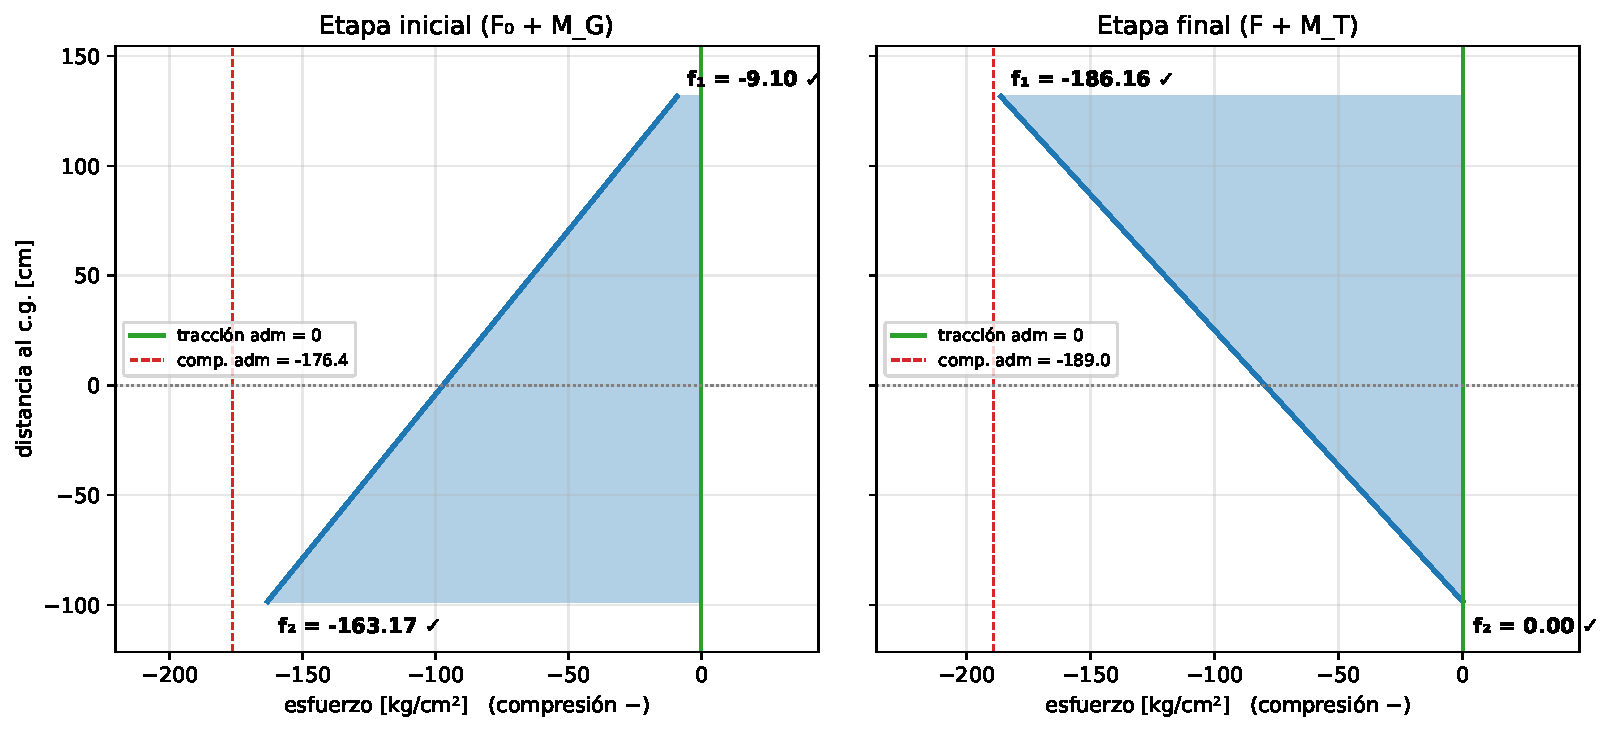
\includegraphics[width=\textwidth]{esfuerzos_L2.pdf}
\caption{Distribución de esfuerzos en $L/2$ con los límites admisibles.}
\end{figure}



\section{Eficiencia de la sección}
\[
Q = \frac{k_1 + k_2}{h} = \frac{64.35 + 48.16}{230.00} = \textbf{0.489}
\qquad
Q = \frac{r^2}{c_1\,c_2} = \frac{6\,335.42}{(131.55)(98.45)} = 0.489
\]
Criterio: $Q = 0.50$ diseño eficiente; $Q < 0.45$ sección pesada; $Q > 0.55$ sección demasiado esbelta.
Resultado: \textbf{Diseño eficiente ($0.45 \le Q \le 0.55$, óptimo $Q = 0.50$)}.


\section{Diseño del cable resultante}
$F_0$, $F$ y $e$ se calcularon en el centro de la luz por ser la zona crítica en vigas simplemente apoyadas.
El cable resultante es una parábola que pasa por la excentricidad $e$ en el centro de la luz y por el centro
de gravedad de la sección en los apoyos.

\subsection{Trayectoria parabólica}
Con origen en el centro de la luz ($X = x - L/2$) y $y$ medido hacia arriba desde el punto más bajo del cable:
\begin{align*}
y &= k\,X^2, \qquad k = \frac{e}{(L/2)^2} = \frac{0.8145\ \text{m}}{(17.50\ \text{m})^2} = 0.002660\ \text{m}^{-1}\\
e(x) &= e\,\frac{4\,x\,(L-x)}{L^2} \quad \text{(excentricidad respecto al c.g.)}\\
\alpha &= k\,L = (0.002660)(35.00) = 0.0931\ \text{rad} = 5.33^\circ \quad \text{(ángulo de salida en el apoyo)}
\end{align*}

\subsection{Curvas límite}
A partir del c.g. se trazan las rectas del núcleo central ($k_1$ hacia arriba y $k_2$ hacia abajo). Con $F_0$ y $F$ constantes:
\begin{align*}
\text{Etapa inicial } (f_1 = 0):\quad & e_{ini}(x) = k_2 + \frac{M_G(x)}{F_0} \qquad \text{(desde la recta de } k_2 \text{ hacia abajo)}\\
\text{Etapa final } (f_2 = 0):\quad & e_{fin}(x) = \frac{M_T(x)}{F} - k_1 \qquad \text{(desde la recta de } k_1 \text{ hacia abajo)}
\end{align*}
Si el cable cumple $e_{fin}(x) \le e(x) \le e_{ini}(x)$, los esfuerzos en las fibras extremas son de compresión en ambas etapas.
En el centro de la luz: $e_{ini} = 48.16 + \dfrac{20\,168\,400}{533\,539.85} = 85.96$ cm y
$e_{fin} = \dfrac{63\,763\,853}{437\,327.75} - 64.35 = 81.45$ cm.

Las curvas límite \textbf{no se cortan}: existe una zona admisible a lo largo de toda la luz. Holgura en $L/2$: $e_{ini} - e_{fin} = 4.51$ cm.

Verificación del cable a lo largo de toda la luz (401 secciones): \textcolor{verde}{\textbf{el cable resultante queda entre las curvas límite en toda la viga.}}

\begin{figure}[H]
\centering
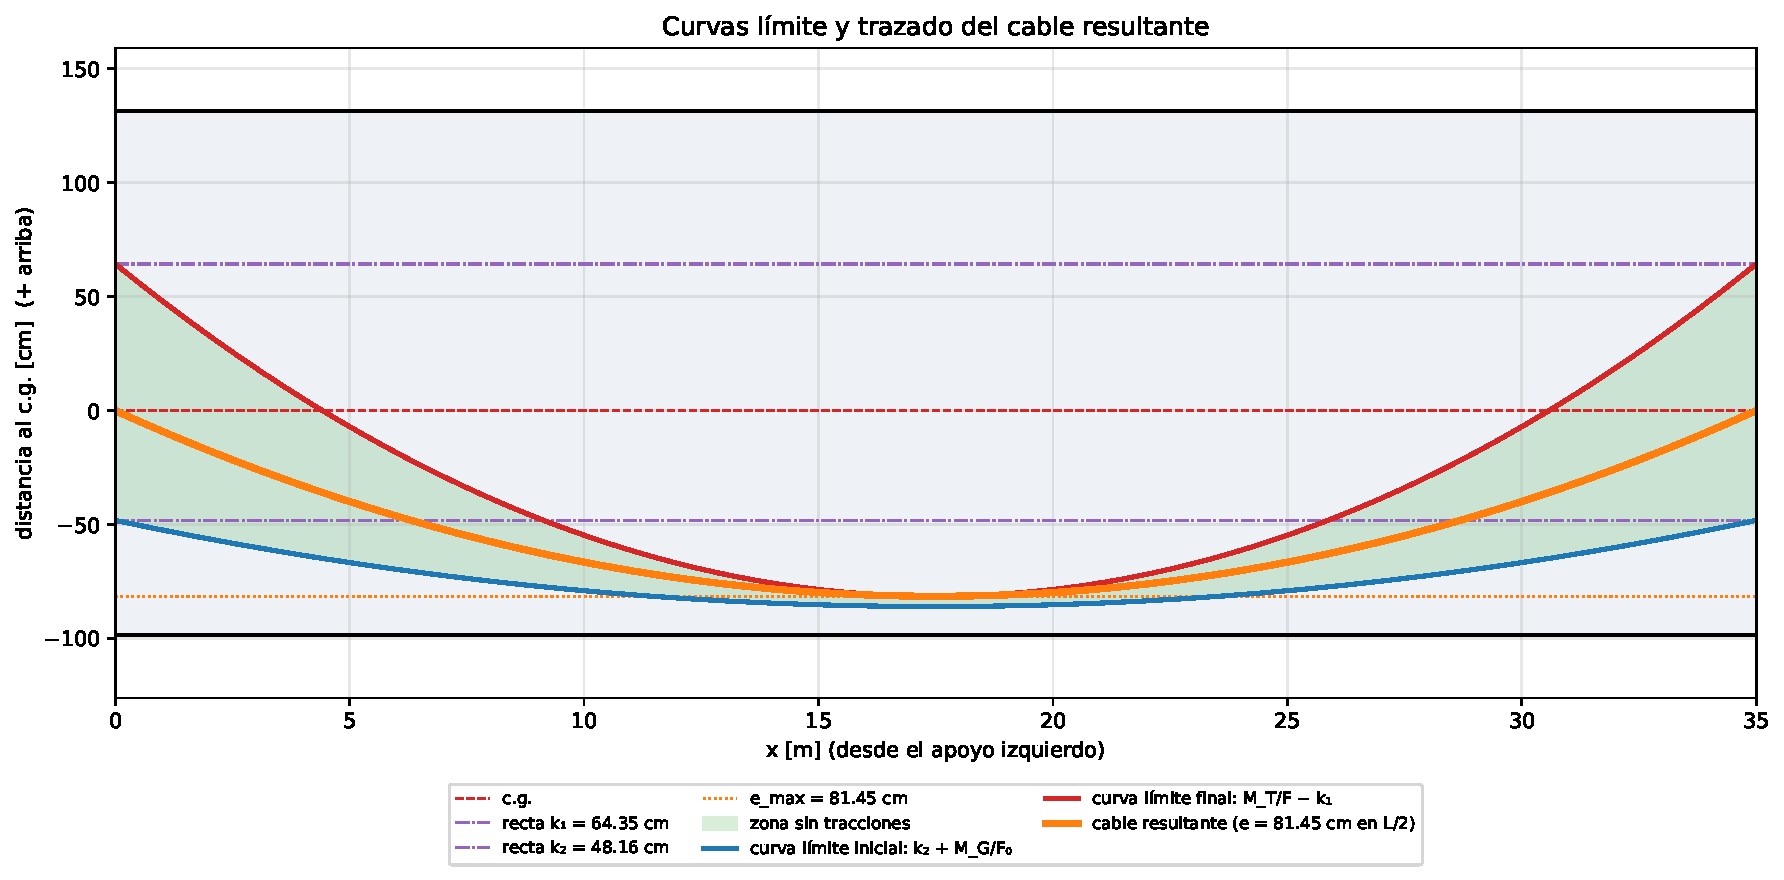
\includegraphics[width=\textwidth]{curvas_limite.pdf}
\caption{Curvas límite inicial y final y trazado del cable resultante.}
\end{figure}



\section{Número y posición de los torones}
Se disponen \textbf{$n = 4$ torones}. Todos llevan la misma fuerza ($F/n$), por lo que la resultante se ubica
en el promedio de sus posiciones y debe coincidir con el cable resultante: en $L/2$ a $y = \bar y - e = 17.00$ cm
y en los apoyos en el c.g., $y = \bar y = 98.45$ cm. Cada torón sigue la parábola $y_i = y_{i,c} + k_i X^2$ con
$k_i = (y_{i,a} - y_{i,c})/(L/2)^2$ y ángulo de salida $\alpha_i = k_i L$.

\begin{center}\footnotesize\setlength{\tabcolsep}{3.5pt}
\begin{tabular}{rrrrrrrrrl}
\toprule
 & \multicolumn{3}{c}{Centro de la luz} & \multicolumn{3}{c}{Apoyo} & & & \\
Torón & $x$ [cm] & $y$ [cm] & $e$ [cm] & $x$ [cm] & $y$ [cm] & $e$ [cm] & $k_i$ [m$^{-1}$] & $\alpha_i$ [$^\circ$] & Dentro \\
\midrule
1 & -4.0 & 10.00 & 88.45 & -4.0 & 84.45 & 14.00 & 0.002431 & 4.88 & \textcolor{verde}{Sí} \\
2 & 4.0 & 10.00 & 88.45 & 4.0 & 84.45 & 14.00 & 0.002431 & 4.88 & \textcolor{verde}{Sí} \\
3 & -4.0 & 24.00 & 74.45 & -4.0 & 112.45 & -14.00 & 0.002888 & 5.79 & \textcolor{verde}{Sí} \\
4 & 4.0 & 24.00 & 74.45 & 4.0 & 112.45 & -14.00 & 0.002888 & 5.79 & \textcolor{verde}{Sí} \\
\bottomrule
\end{tabular}
\end{center}

\textbf{Resultante en el centro de la luz:}
\begin{align*}
\bar y_c &= \frac{\Sigma y_{i,c}}{n} = \frac{10.00 + 10.00 + 24.00 + 24.00}{4} = 17.00\ \text{cm}\\
e_{res} &= \bar y - \bar y_c = 98.45 - 17.00 = 81.45\ \text{cm}
\qquad (\text{diseño: } e = 81.45\ \text{cm},\ \Delta = 0.000\ \text{cm})
\end{align*}
\textbf{Resultante en el apoyo:}
\begin{align*}
\bar y_a &= \frac{\Sigma y_{i,a}}{n} = \frac{84.45 + 84.45 + 112.45 + 112.45}{4} = 98.45\ \text{cm}\\
e_{res} &= \bar y - \bar y_a = 98.45 - 98.45 = 0.00\ \text{cm}
\qquad (\text{debe ser } 0,\ \Delta = 0.005\ \text{cm})
\end{align*}
Tolerancia adoptada: $\pm 0.50$ cm. Resultante: \textcolor{verde}{coincide con el cable resultante}. Torones dentro del hormigón en toda la luz: \textcolor{verde}{sí}.

\begin{figure}[H]
\centering
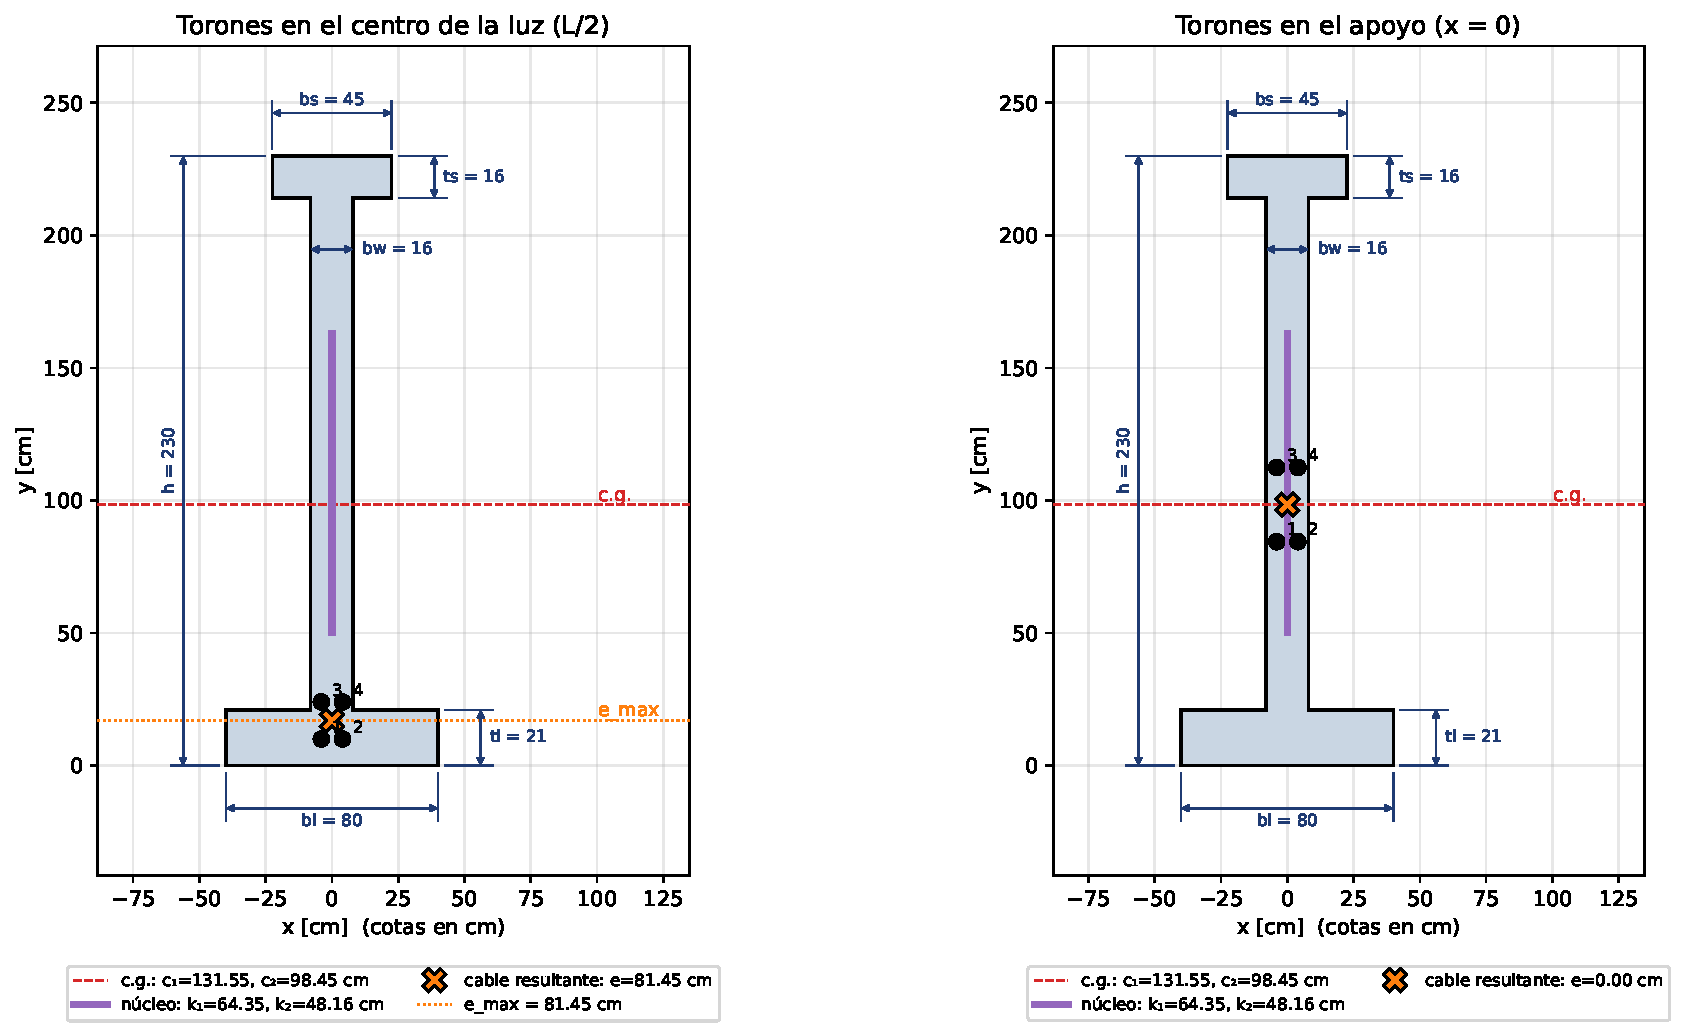
\includegraphics[width=\textwidth]{torones_secciones.pdf}
\caption{Posición de los torones en el centro de la luz y en el apoyo.}
\end{figure}


\begin{figure}[H]
\centering
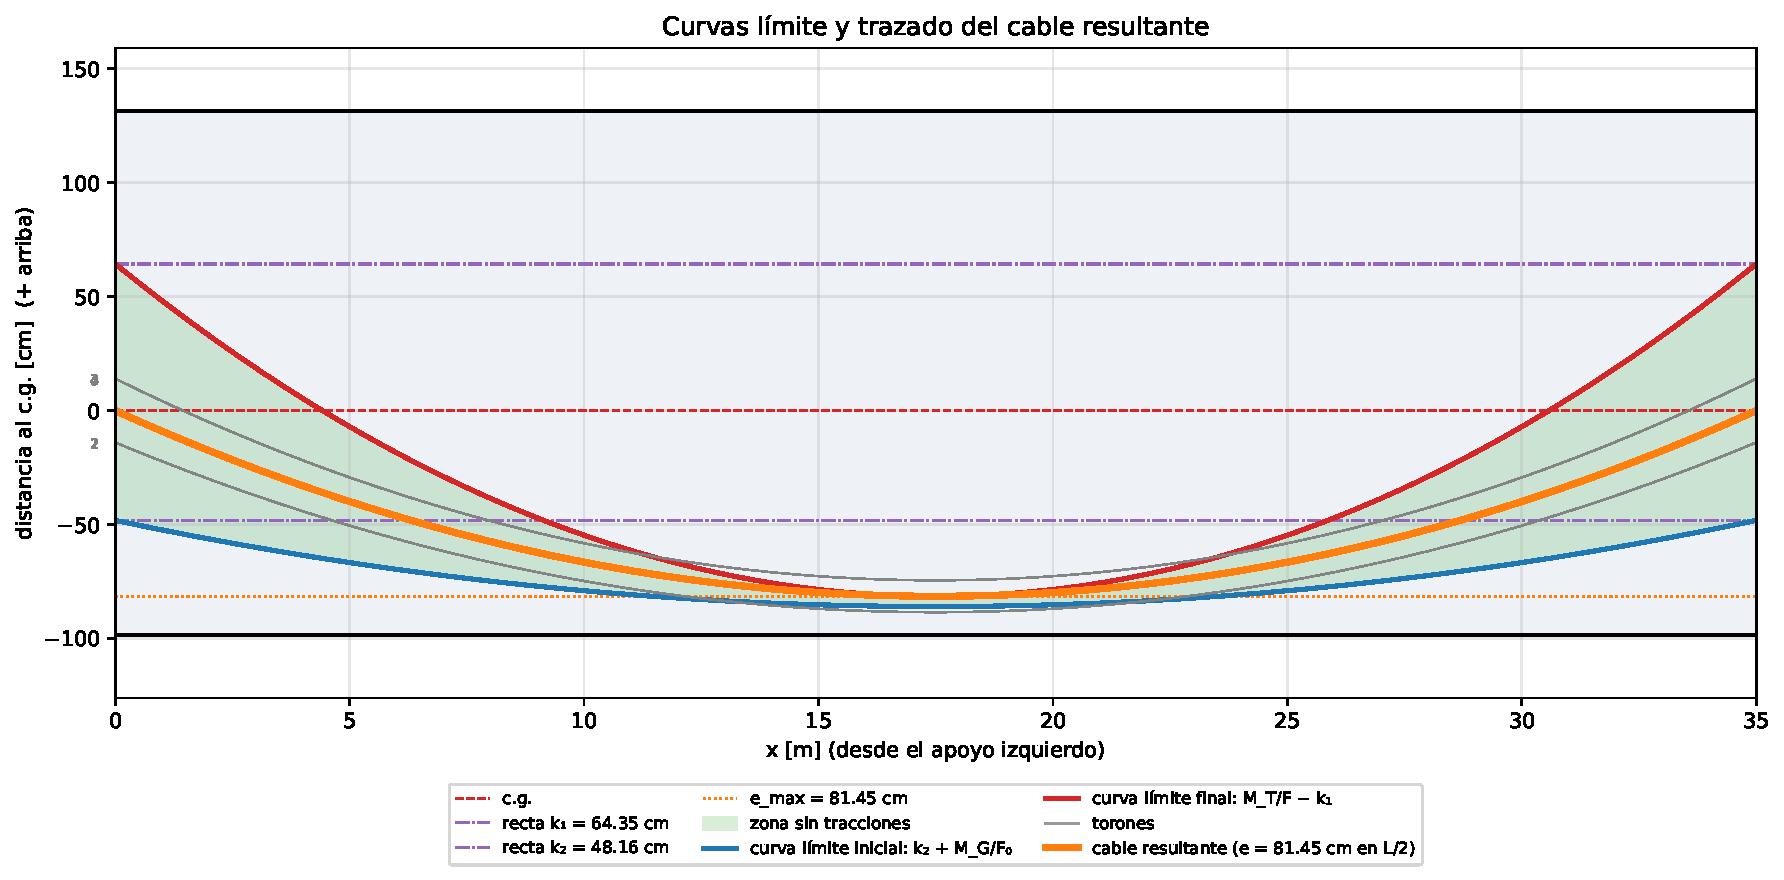
\includegraphics[width=\textwidth]{torones_elevacion.pdf}
\caption{Trayectoria de los torones y del cable resultante entre las curvas límite.}
\end{figure}



\section{Conclusión}
\begin{center}
\begin{tabular}{>{\raggedright\arraybackslash}p{9cm}ll}
\toprule
Verificación & Tipo & Estado \\
\midrule
Esfuerzos admisibles en $L/2$ (tracción = 0) & Obligatoria & \textcolor{verde}{Cumple} \\
Cable resultante entre las curvas límite en toda la luz & Obligatoria & \textcolor{verde}{Cumple} \\
Resultante de los torones coincide con el cable resultante & Obligatoria & \textcolor{verde}{Cumple} \\
Torones dentro del hormigón & Obligatoria & \textcolor{verde}{Cumple} \\
Eficiencia $0.45 \le Q \le 0.55$ (criterio de economía) & Recomendación & \textcolor{verde}{Cumple} \\
Área de hormigón $\ge A_{c,req}$ (predimensionamiento) & Recomendación & \textcolor{verde}{Cumple} \\
\bottomrule
\end{tabular}
\end{center}
\begin{itemize}
\item Sección adoptada: I  (bs=45, ts=16, bw=16, bi=80, ti=21, h=230), $h = 230.0$ cm, $A = 5\,488.00$ cm$^2$ ($q_G = 1\,317.12$ kg/m).
\item Presfuerzo: $F_0 = 533\,539.85$ kg, $F = 437\,327.75$ kg, excentricidad restringida $e = 81.45$ cm en $L/2$.
\item Cable resultante parabólico $y = 0.002660\,X^2$ (m), ángulo de salida $\alpha = 5.33^\circ$.
\item Torones: $n = 4$.
\end{itemize}
\begin{center}\Large \textcolor{verde}{\textbf{DISEÑO VÁLIDO}}\end{center}
\end{document}
